%
% 4fAufbau.tex -- Bild zum Thema Optische Fouriertransformation <opt>
%
% (c) 2023 Marco Niederberger, Yanick Schoch; OST Ostschweizer Fachhochschule
%

\documentclass[tikz]{standalone}
\usepackage{txfonts}
\usepackage{pgfplots}

\pgfplotsset{compat=1.16}
\def\skala{1}

\usetikzlibrary{arrows,intersections,math}
\usetikzlibrary{decorations.markings, calc}

%% Lense (x, height, curvature)
\newcommand{\lense}[3]{
    \def\curvature{0.2}
    \path[fill=glass, draw=black, line width = 0.6, opacity=0.8] (#1,-#2) .. controls (#1 - #3,0) .. (#1,#2) .. controls (#1 + #3,0) .. (#1,-#2);
}

%% Axis (x, textAbove, textBelow)
\newcommand{\xAxis}[3]{%
    \def\lenseX{3.5}
    \draw[->, thin] (#1,-\lenseX)--(#1,\lenseX) node[above]{#2};
    \node[] at (#1, -\lenseX - 0.5){#3};
}

%% Dimension arrow (xStart, xEnd)
\newcommand{\dimensionBetweenLenses}[2]{%
    \def\dimensionHeight{-3.3}
    \draw[<->] (#1, \dimensionHeight)--(#2, \dimensionHeight) node[above,midway] {$f$};
}

% Styles
%% Arrow in the Middle
\tikzset{arrow inside/.style = {postaction=decorate,decoration={markings,mark=at position 0.52 with \arrow{stealth}}}}

% Define Color
\definecolor{glass}{cmyk}{0.2,0,0,0}

\begin{document}

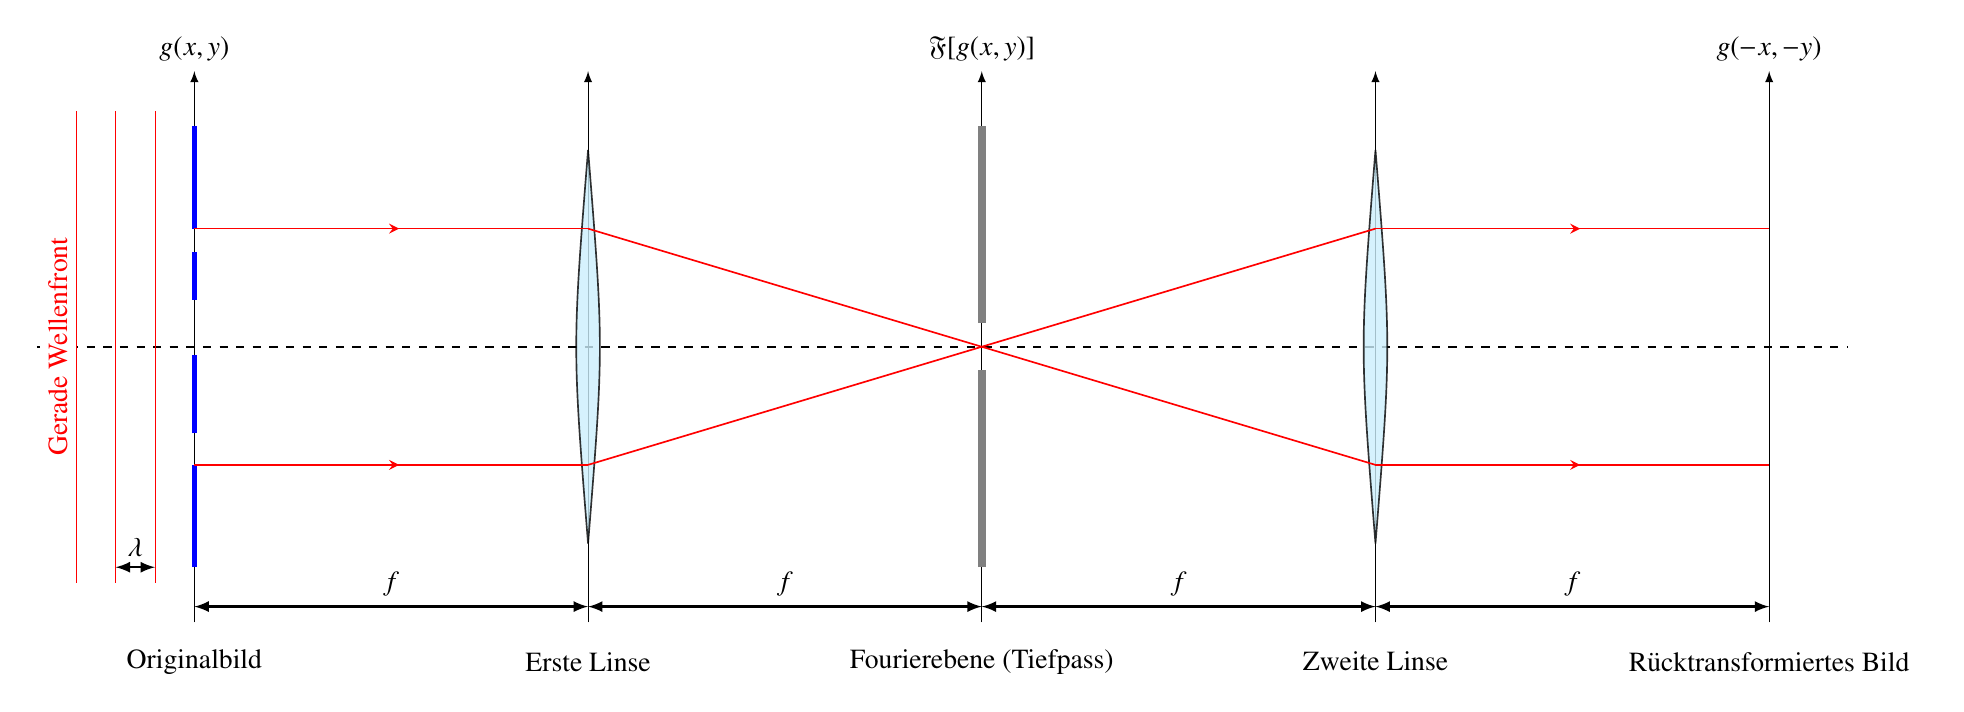
\begin{tikzpicture}[>=latex,thick,scale=\skala]

    % Force the boundary to be symmetric around (0,0)
    \node[] at (-12,0){};
    \node[] at (12,0){};

    % xAxis
    \xAxis{-10}{$g(x,y)$}{Originalbild}
    \xAxis{-5}{}{Erste Linse}
    \xAxis{0}{$\mathfrak{F}[g(x,y)]$}{Fourierebene (Tiefpass)}
    \xAxis{5}{}{Zweite Linse}
    \xAxis{10}{$g(-x,-y)$}{Rücktransformiertes Bild}

    % Optical plane
    \draw[dashed] (-12,0)--(11,0);

    % Dimension between the lenses
    \foreach \n in {-2,...,1}{
        \dimensionBetweenLenses{\n * 5}{\n * 5 + 5}
    }

    % Lenses
    \lense{-5}{2.5}{.2}
    \lense{5}{2.5}{.2}

    % Aperture
    \draw[-, line width=2, blue] (-10,-2.8)--(-10,-1.5);
    \draw[-, line width=2, blue] (-10,-1.1)--(-10,-0.1);
    \draw[-, line width=2, blue] (-10,0.6)--(-10,1.2);
    \draw[-, line width=2, blue] (-10,1.5)--(-10,2.8);

    % Laser wave
    \draw[<->] (-11, -2.8)--(-10.5,-2.8) node[above,midway] {$\lambda$};
    \draw[-, red, line width = 0.3] (-11.5, -3)--(-11.5,3) node[above,midway, sloped, fill=white, inner sep = 3] {Gerade Wellenfront};
    \draw[-, red, line width = 0.3] (-11, -3)--(-11,3);
    \draw[-, red, line width = 0.3] (-10.5, -3)--(-10.5,3);

    % Low pass filter
    \draw[-, line width=3, gray] (0,-2.8)--(0,-0.3);
    \draw[-, line width=3, gray] (0,0.3)--(0,2.8);

    % Rays
    \draw[red, line width = 0.6, arrow inside] (-10,1.5) -- (-5,1.5);
    \draw[red, line width = 0.6] (-5,1.5) -- (5,-1.5);
    \draw[red, line width = 0.6, arrow inside] (5,-1.5) -- (10,-1.5);

    \draw[red, line width = 0.6, arrow inside] (-10,-1.5) -- (-5,-1.5);
    \draw[red, line width = 0.6] (-5,-1.5) -- (5,1.5);
    \draw[red, line width = 0.6, arrow inside] (5,1.5) -- (10,1.5);

\end{tikzpicture}
\end{document}

